%-------------------------------------------------------------------------
% INFORMACIÓN DEL ARTÍCULO
\thispagestyle{portadapage}
\setcounter{subsection}{0}
\setcounter{subsubsection}{0}
\setcounter{actividad}{0}
\setcounter{actividad_previa}{0}
\setcounter{actividad_entre}{0}
\renewcommand{\articulotipo}{Comunicación breve}
\renewcommand{\articulotitulo}{Múltiples registros con los axiomas de incidencia de la geometría euclidiana}
\phantomsection
\stepcounter{section}
\addcontentsline{toc}{section}{\protect\numberline{\thesection} \articulotitulo}
\desctotoc{Sángari, A. N.}

\begin{center}
	\setstretch{1.5}
	{\Huge \scshape 
		\articulotitulo
	}
\end{center}

\noindent\rule{\linewidth}{2pt}

\vspace{0.25cm}

\begin{flushright}
	{\Large \scshape
		Antonio Noé Sángari
	}\\
	{\large \itshape
		Universidad Nacional de Salta
	}\\
	{\ttfamily \small
		jem@exa.unsa.edu.ar
	}\\
\end{flushright}

\vspace{0.5cm}

\begin{center}
	\begin{minipage}{0.75\linewidth} \small
		\textsc{Resumen}. ~
		Este trabajo explora el concepto de registros en geometría, entendidos como diferentes formas de representar y comunicar conceptos geométricos. Estos registros incluyen lingüísticos (uso de lenguaje verbal), gráficos (dibujos y diagramas), simbólicos (símbolos matemáticos), manipulativos (uso de materiales físicos) y computacionales (uso de software). Luego, se destaca la importancia del registro simbólico en la lógica y geometría.
		
		El uso del registro simbólico aporta profundidad al concepto, permitiendo abstracción y generalización. También ofrece rigor y precisión mediante el lenguaje formal y las reglas lógicas. La relación con la lógica es estrecha, ya que el registro simbólico se basa en principios lógicos y fomenta la comprensión de la lógica y la geometría. La demostración de un axioma de incidencia se muestra como un ejemplo de cómo el registro simbólico facilita el razonamiento y la comprensión de los conceptos.
		
		Además, se menciona que la lógica puede abordarse como un juego sintáctico, lo que la hace más accesible y atractiva para principiantes en matemáticas. Esta aproximación enfatiza en las reglas y estructura, se relaciona con el pensamiento abstracto y permite una exploración gradual y experimentación.
	\end{minipage}\\
	
	\vspace{0.5em}
	
	\begin{minipage}{0.75\linewidth} \small
	\textsc{Palabras clave} --- Registros en geometría, Representación geométrica, Enseñanza de matemáticas, Experimentación en lógica y geometría, Comprensión geométrica.
	\end{minipage}
\end{center}
%-------------------------------------------------------------------------

\subsection{Introducción}

\subsubsection{Importancia del trabajo con varios registros}

Entenderemos a los registros en geometría como las diferentes formas en que se pueden representar y comunicar los conceptos y procesos geométricos. Los registros son sistemas semióticos que permiten la expresión y el intercambio de ideas geométricas entre los estudiantes, los docentes y los materiales de enseñanza. Ver \textcite{duval1999semiosis}

Los registros en la geometría pueden incluir:
\begin{itemize}
	\item Registros lingüísticos: El uso del lenguaje natural, incluyendo términos, definiciones, proposiciones y argumentos geométricos expresados en palabras.
	\item Registros gráficos: El uso de dibujos, diagramas, esquemas y representaciones visuales para ilustrar y comunicar ideas geométricas.
	\item Registros simbólicos: El uso de símbolos matemáticos y notación algebraica para expresar relaciones y propiedades geométricas.
	\item Registros manipulativos: El uso de materiales físicos, como modelos geométricos, construcciones con regla y compás, o manipulación de objetos tridimensionales, para explorar y experimentar con conceptos geométricos.
	\item Registros computacionales: El uso de software de geometría dinámica, como Geogebra, para visualizar y manipular objetos geométricos, realizar construcciones interactivas y realizar cálculos relacionados con la geometría.
\end{itemize}

El tratamiento de los registros en los axiomas de incidencia de la geometría euclidiana es importante porque nos permite comprender y comunicar de manera efectiva los conceptos y propiedades geométricas. Aquí hay algunas razones clave por las cuales el tratamiento de los registros es relevante en este contexto:
\begin{description}
	\item[Claridad y comprensión] Los diferentes registros ofrecen diferentes formas de representar y comprender los axiomas de incidencia. Al utilizar registros lingüísticos, gráficos, simbólicos y manipulativos, podemos abordar los axiomas desde múltiples perspectivas, lo que facilita la comprensión de los conceptos geométricos involucrados.
	\item[Comunicación efectiva] Los registros nos permiten comunicar los axiomas de incidencia de la geometría euclidiana de manera clara y precisa. Cada registro tiene su propio lenguaje y conjunto de convenciones, lo que permite una comunicación más efectiva entre estudiantes, docentes y materiales de enseñanza.
	\item[Representación visual] Los registros gráficos y manipulativos, como diagramas, modelos físicos y construcciones geométricas, permiten una representación visual de los axiomas. Esto ayuda a los estudiantes a visualizar y comprender mejor las relaciones espaciales y las propiedades geométricas.
	\item[Abstracción y generalización] El uso de registros simbólicos y lingüísticos, como fórmulas matemáticas y definiciones formales, permite la abstracción y generalización de los axiomas de incidencia. Estos registros nos permiten expresar los axiomas de manera concisa y formal, lo que facilita su aplicación en diferentes contextos geométricos.
	\item[Flexibilidad y transferencia] Al trabajar con diferentes registros, los estudiantes pueden desarrollar habilidades de flexibilidad y transferencia conceptual. Pueden aprender a traducir y relacionar los conceptos geométricos entre diferentes registros, lo que les permite aplicar su conocimiento en una variedad de situaciones geométricas.
\end{description}

En este trabajo presentaremos breves comentarios sobre el uso de múltiples registros para la enseñanza de los axiomas de incidencia de la geometría euclidiana, pero enfatizando el registro simbólico. 

\subsection{Requisitos previos}

Entendimiento básico de la lógica proposicional y el razonamiento deductivo. Conceptos básicos de Geometría Euclidiana.

\subsection{Desarrollo}

\subsubsection{Comentarios sobre el problema teórico}

El conjunto de símbolos propios de la teoría \textbf{IGE} de Incidencia de la Geometría Euclidiana son $\{ =, \mathcal{P}(), \mathcal{R}(), \pi(), \mathcal{I}_{\mathcal{R}}(), \mathcal{I}_{\pi}() \}$. Esto quiere decir que debo escribir esta teoría usando solamente estos símbolos y otros símbolos de la lógica. Por costumbre, a las variables se las escribe con letras mayúsculas de imprenta, si se quiere hacer alusión a puntos, con letras minúsculas de imprenta si se quiere hacer alusión a rectas, y con letras griegas minúsculas si se quiere hacer alusión a planos. $\mathcal{P}(A)$ se lee <<$A$ es un punto>>, $\mathcal{R}(s)$, <<$s$ es una recta>>, $\pi(\nu)$ <<$\nu$ es un plano>>, $\mathcal{I}_{\mathcal{R}}(P,m)$ <<El punto $P$ está en incidencia con la recta $m$>> o <<$m$ pasa por $P$>> o <<$P$ está en $m$>>, etc; y similarmente para $\mathcal{I}_{\pi}(P,\alpha)$. Para acortar la notación, un pequeño abuso de notación permitido es $\mathcal{P}(A,B,C)$ lo entendemos por $\mathcal{P}(A) \wedge \mathcal{P}(B) \wedge \mathcal{P}(C)$ y similarmente para $\mathcal{R}()$, $\pi()$. También escribimos $A,B,C \in r$ en cuenta de $\mathcal{I}_{\mathcal{R}}(A,r) \wedge \mathcal{I}_{\mathcal{R}}(B,r) \wedge \mathcal{I}_{\mathcal{R}}(C,r)$ y $A,B,C \in \alpha$ en cuenta de $\mathcal{I}_{\pi}(A,\alpha) \wedge \mathcal{I}_{\pi}(B,\alpha) \wedge \mathcal{I}_{\pi}(C,\alpha)$, siempre que esto no lleve a ambigüedad. Ver \textcite{margaris1990first11}

\begin{observacion}
	La pregunta que puede surgir es ¿Cuál es el valor agregado del uso del registros simbólico? Se puede responder de dos maneras: Primero, tiene una gramática muy simple (en comparación a los lenguajes naturales como el inglés o el español). Segundo, es un problema sintáctico, y por lo tanto, los pasos en una deducción son solamente manipulación de cadenas.
	
	Para entender mejor el segundo punto en la observación anterior vamos a considerar lo siguiente: Si en cuenta de leer $\mathcal{P}(A)$ como <<$A$ es un punto>> se lo leyera como <<$A$ es un jugador de futbol>>, $\mathcal{R}(s)$ como <<$s$ es una recta>> se lo leyera como <<$s$ es un equipo de futbol>> , $\pi(\nu)$ se lo leyera como <<$\nu$ es un plano>>, $\mathcal{I}_{\mathcal{R}}(P,m)$ <<El punto $P$ está en incidencia con la recta $m$>> o <<$m$ pasa por $P$>> o <<$P$ está en $m$>>, etc; y similarmente para $\mathcal{I}_{\pi}(P,\alpha)$.
\end{observacion}

\subsubsection{Ejemplo ilustrativo}

Consideremos el primer axioma de incidencia según la formulación de \textcite{efimov1984geometria11}: <<Cualesquiera que sea el punto $A$ y cualesquiera que sea el punto $B$, existe una recta $a$ que pasa por $A$ y por $B$>>. 
\begin{itemize}
	\item Registro lingüístico: Podemos expresar el axioma utilizando lenguaje verbal, por ejemplo: <<Cualesquiera que sea el punto $A$ y cualesquiera que sea el punto $B$, existe una recta $a$ que pasa por $A$ y por $B$>>.
	\item Registro gráfico: Podemos representar el axioma mediante un diagrama que muestra dos puntos $A$ y $B$ y una línea que los conecta. Ver figura \ref{fig:Axioma-I-de inciden}
	
	\begin{figure}[h!]
		\centering
		\caption{}
		\label{fig:Axioma-I-de inciden}
		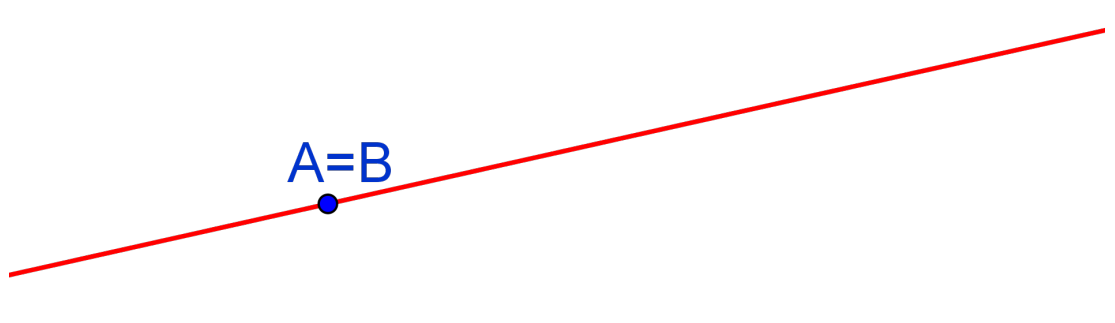
\includegraphics[scale=0.2]{Trabajos/11/Envios/Ax1a.PNG}
		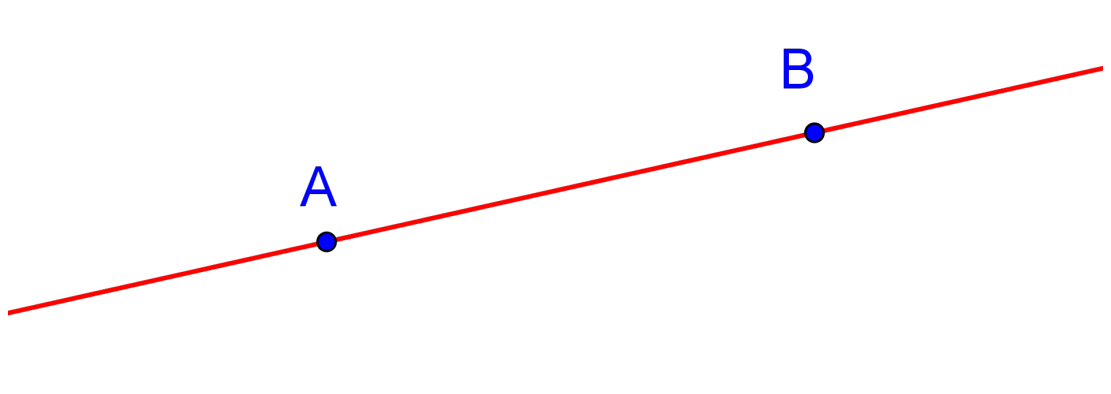
\includegraphics[scale=0.2]{Trabajos/11/Envios/Ax1b2b.PNG}
	\end{figure}
	
	\item Registro simbólico: Podemos usar símbolos matemáticos para expresar el axioma, por ejemplo: $\forall A \forall B \exists r \bigl( P(A,B) \rightarrow \mathcal{R}(r) \wedge A,B \in r \bigr)$
	
	\item Registro manipulativo: Podemos utilizar regla y compás para construir físicamente una línea que pase por los puntos $A$ y $B$.
	
	\item Registros computacionales: Con el uso de Geogebra, se puede realizar dibujos dinámicos, es decir que en este caso pudiera cambiarse las posiciones relativas de $A$ y de $B$ y ver el cambio de la línea que pasa por $A$ y por $B$. Para más ejemplos de este recurso puede verse \cite{geometria11congeogebra11}.
\end{itemize}

Es común interpretar de la representación lingüística de este axioma que los puntos $A$ y $B$ son distintos. En esta formulación de los axiomas de incidencia, no se especifica explícitamente que los puntos $A$ y $B$ deben ser distintos y, por lo tanto, permite la posibilidad de que $A$ y $B$ sean el mismo punto. Sin embargo, en el caso de la representación simbólica, y con un pequeño auxilio de la lógica, se despejan las dudas. Por ejemplo, revisando la siguiente demostración con el uso del registro simbólico queda claro una implicación de este axioma:
\begin{teorema}
	Si existe un punto, existe una recta: $\vdash\exists A \mathcal{P}(A) \rightarrow \exists r \mathcal{R}(r)$
\end{teorema}

\begin{proof}
	~
	
	\begin{center}
		\def\arraystretch{1.5}
		\begin{tabular}{|c|l|c|}
			\hline 
			1. & $\exists A \mathcal{P}(A)$ & as\\
			\hline 
			2. & $\mathcal{P}(A)$ & c$A$\\
			\hline 
			3. & $\forall A \forall B \exists r \bigl( \mathcal{P}(A,B) \leftarrow \mathcal{R}(r) \wedge A,B \in r \bigr)$ & ax1\\
			\hline 
			4. & $\exists \bigl( \mathcal{P}(A,A) \leftarrow \mathcal{R}(r) \wedge A,A \in r \bigr)$ & spec\\
			\hline 
			5. & $\mathcal{P}(A,A) \rightarrow \mathcal{R}(r) \wedge A,A, \in r$ & c$r$\\
			\hline 
			6. & $\mathcal{R}(r)$ & SC 2,5\\
			\hline 
			7. & $\exists r \mathcal{R}(r)$ & $\exists$\\
			\hline 
			8. & $\exists r \mathcal{R}(r)$ & c5\\
			\hline 
			9. & $\exists r \mathcal{R}(r)$ & c2\\
			\hline 
			10. & $\exists A \mathcal{P}(A) \rightarrow \exists r \mathcal{R}(r)$ & DT 1-9\\
			\hline 
		\end{tabular}
	\end{center}
	
\end{proof}

En esta demostración solamente usamos el axioma propio 1, además de metateoremas del cálculo de predicados con la igualdad. Una explicación puede ser la siguiente:
\begin{enumerate}
	\item Se supone la existencia de un punto $A$ ($\exists A$) y se afirma que es un punto ($\mathcal{P}(A)$).
	\item Se introduce la notación “cA” para denotar el uso de la regla $C$.
	\item Se utiliza el primer axioma de incidencia.
	\item Se realiza una instancia de cuantificador universal, reemplazando $B$ por $A$ en el axioma, es decir especializando el axioma.
	\item Se utiliza nuevamente la regla C pero esta vez en $r$.
	\item Se utiliza un silogismo o un teorema del calculo de proposiciones (SC) para concluir que $r$ es una recta.
	\item Se utiliza la introducción del cuantificador existencial para afirmar que existe una recta $r$. 
	\item Se descarga la regla C aplicada a $r$.
	\item Se descarga la regla C aplicada a $A$.
	\item Se aplica el teorema de la deducción y se concluye.
\end{enumerate}

\subsection{Bibliografía}

% \nocite{*}
\printbibliography[keyword={11}]